% Appendix fragment: depth-boundary material -- transport measurement, depth structure,
% mechanism interventions, and late-depth behaviour. Included from appendix.tex via
% % Appendix fragment: depth-boundary material -- transport measurement, depth structure,
% mechanism interventions, and late-depth behaviour. Included from appendix.tex via
% % Appendix fragment: depth-boundary material -- transport measurement, depth structure,
% mechanism interventions, and late-depth behaviour. Included from appendix.tex via
% % Appendix fragment: depth-boundary material -- transport measurement, depth structure,
% mechanism interventions, and late-depth behaviour. Included from appendix.tex via
% \input{appendix_depth}.

\section{The transport measurement in full}\label{app:transport}

A forward pre-hook on every decoder layer adds $-10^4$ to the attention logits of chosen query rows over the
image-token columns, at chosen layers only. Masking \emph{all} text rows at \emph{all} layers destroys the answer
(KL $1.266$ / $0.532$, $42\%$ / $45\%$ of answers flip, $n{=}40$); masking only the answer token's row at all layers
does not (KL $0.025$, $3\%$ flip). Table~\ref{tab:prefix} localises the window.


\begin{figure}[h]\centering
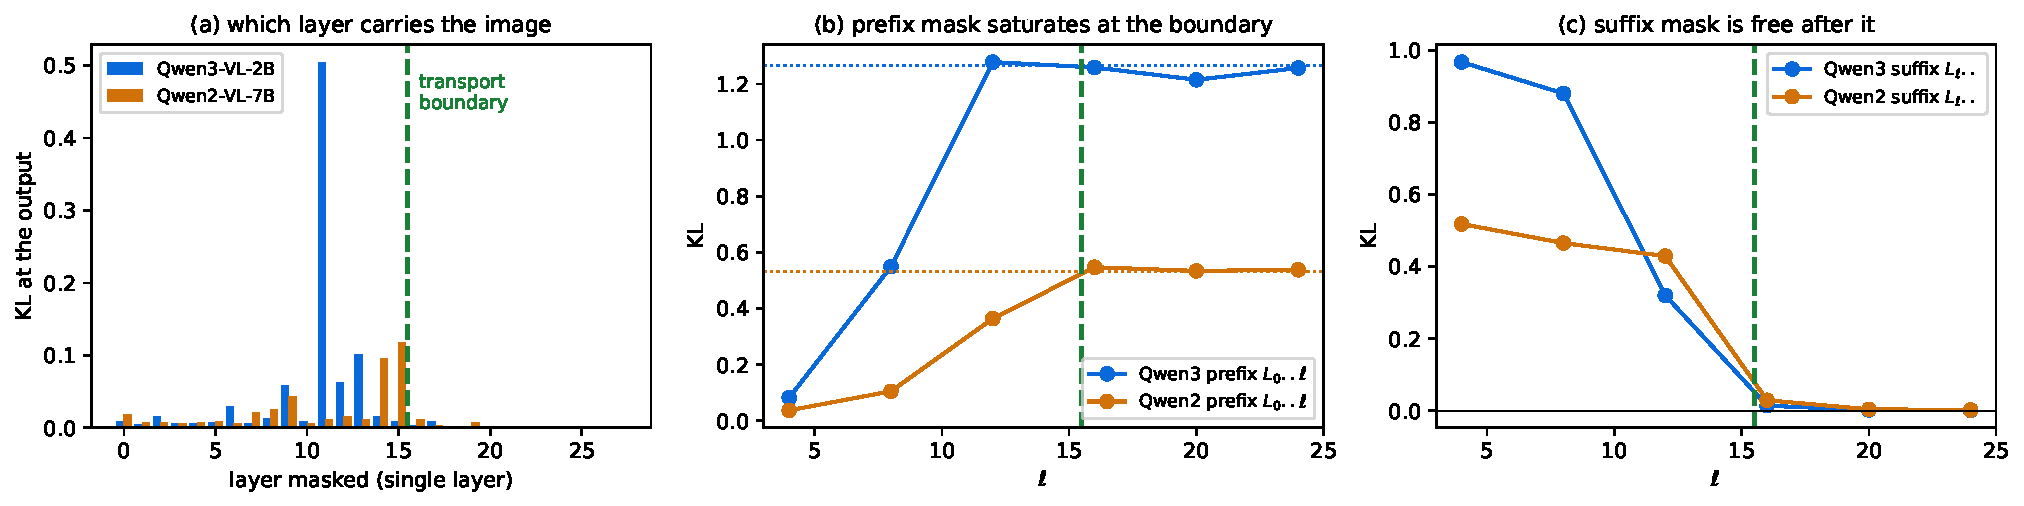
\includegraphics[width=\textwidth]{figs/fig_transport.pdf}
\caption{\textbf{The transport measurement.} (a) Masking one layer's image attention at a time: the effect is
concentrated well before the boundary and is at or below $0.0023$ from L20 on both models. (b) Masking a prefix
$L_0..\ell$ reaches the full-mask value (dotted) once $\ell$ passes the window. (c) Masking a suffix
$L_\ell..\text{end}$ costs nothing once $\ell$ is past it. Three readings, one boundary.}
\label{fig:transport}
\end{figure}

Single-layer masks peak at L11 on Qwen3 (KL $0.504$; next highest L13 at $0.101$) and at L15/L14 on Qwen2
($0.118$/$0.096$). From L20 onward every layer is at or below $0.0023$ on both models. On Qwen3-VL-8B, which has
$36$ layers, the same behaviour appears at L21, i.e.\ the same $0.57$ fraction of depth.

\paragraph{Three independent readings of the same boundary.} The masks are one. Pruning is the second: discarding
$90\%$ of visual tokens at the boundary costs $+0.0$ to $+0.5$ points across ten stratum-cells, whereas moving the
same cut to $\ell{=}4$ costs $5.2$ more on one model ($0.5$ on the other), and a taper that removes half the tokens
at $\ell{=}9$--$12$ loses $3.5$ points against not pruning at matched tokens while buying nothing over a single cut
($-1.0$). Read-out depth is the third: restricting the localiser to layers $\le$ L20 costs $-0.5$ and $+1.6$ points
of coverage, while restricting it to $\le$ L16 costs $9.4$ and $22.0$. Transport finishes at the boundary; the
signal the ranking reads is produced after it.

\section{Depth structure across checkpoints}\label{app:depth}

\begin{table}[h]\centering\small
\caption{Where each quantity falls, per checkpoint. The transport boundary and the read-out band are fractions of
depth, not fixed layer indices, which is what lets both policies transfer to a $36$-layer model unchanged. The
$36$-layer boundary is masked: its suffix is harmless at L20 and zero from L24, the same fractions as the pair.}
\begin{tabular}{lccccc}
\toprule
checkpoint & layers & block-mean band & read-out band & boundary & boundary / depth\\
\midrule
Qwen3-VL-2B & 28 & L16--L26 & L17--L20 & L16 & 0.57\\
Qwen2-VL-7B & 28 & L15--L26 & L19--L22 & L16 & 0.57\\
Qwen2.5-VL-7B & 28 & L16--L26 & --- & L16 & 0.57\\
Qwen3-VL-8B & \textbf{36} & L20--L33 & --- & \textbf{L21} & 0.57\\
\bottomrule
\end{tabular}\label{tab:depth}
\end{table}

\section{Mechanism: three stages, three interventions}\label{app:mech}

\begin{figure}[h]\centering
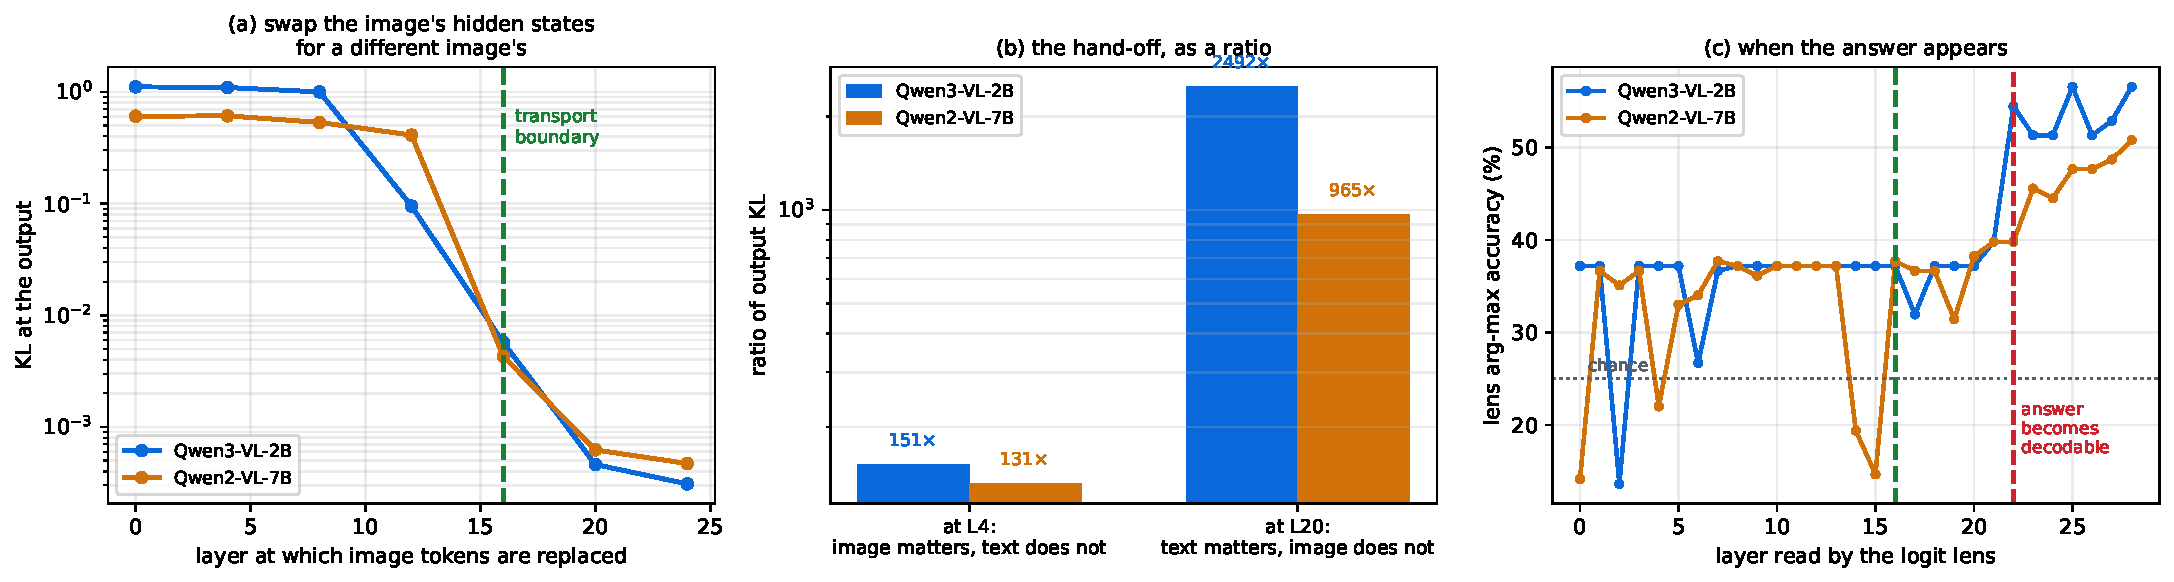
\includegraphics[width=\textwidth]{figs/fig_mechanism.pdf}
\caption{\textbf{(a)} Replacing the image tokens' hidden states at layer $\ell$ with a different image's: the
output effect falls three orders of magnitude across the boundary. \textbf{(b)} The hand-off as a ratio: early,
the image dominates and the text is inert; late, exactly the reverse. \textbf{(c)} Logit lens at the answer
position: the correct option becomes decodable only in the last quarter of the stack.}
\label{fig:mech}
\end{figure}

Each row of Table~\ref{tab:stages} is measured by a different intervention, so no stage rests on the method that
found another.

\begin{table}[h]\centering\small
\caption{The three stages. Every number is measured on both core checkpoints.}
\setlength{\tabcolsep}{4pt}\begin{tabular}{p{2.2cm}p{1.35cm}p{2.8cm}p{5.5cm}}
\toprule
stage & layers & measured by & evidence\\
\midrule
image $\to$ text transport & L0--L16 & attention masking; hidden-state patching & suffix masks cost nothing from L16 ($0.014$, $0.029$); the patch effect falls $17\times$ and $96\times$ between L12 and L16\\
question-conditioned read-out & L17--L21 & end-task accuracy by read-out depth & crop accuracy spans $34.6$--$70.2$, peaking at L17; no layer inside the window beats not cropping\\
answer formation & L22+ & logit lens & lens accuracy steps $+18.0$ [$+8.7,+27.0$] and $+14.2$ [$+7.2,+21.3$] above its early plateau\\
\bottomrule
\end{tabular}\label{tab:stages}
\end{table}

The logit lens is computed with the final norm applied to intermediate layers only; applying it to the last hidden
state as well double-normalises and corrupts that layer alone, which cost us a retracted result earlier in this
project. We assert per run that our last-layer read-out matches the true logits.

A fourth, independent technique places the read-out band in the same spot: a ridge probe from the
answer-position state to the target's location rises across the transport window and peaks at L18--19 (Qwen3,
$r=+0.635$) and L18 (Qwen2, $+0.603$).

\paragraph{The channel and the values.} Masking blocks the text$\to$image attention \emph{channel}; it does not
show that the image information is absent from the residual stream. Replacing the image tokens' hidden states
with a donor image's (same question, same token budget) closes that gap. The effect falls three orders of
magnitude across the boundary, and both pre-registered controls behave as required: patching the image at L4 is
large, patching text at L20 is large.

\begin{table}[t]
\caption{Representation patching: replace the image tokens' hidden states at one layer's output with a donor
image's; KL at the output and answer flips. Text controls patch text-token states at the same depth.}
\label{tab:patch}
\begin{center}
\small
\begin{tabular}{lcc}
\multicolumn{1}{c}{\bf patch site} &\multicolumn{1}{c}{\bf Qwen3-VL-2B KL (flips)} &\multicolumn{1}{c}{\bf Qwen2-VL-7B KL (flips)}
\\ \hline \\
image L0 & 1.758 (61.7\%) & 0.800 (60.0\%)\\
image L4 (control C1) & 1.766 (63.3\%) & 0.798 (58.3\%)\\
image L8 & 1.622 (60.0\%) & 0.657 (60.0\%)\\
image L12 & 0.134 (16.7\%) & 0.517 (51.7\%)\\
image L16 & 0.009 (3.3\%) & 0.005 (5.0\%)\\
image L20 & 0.0005 (0\%) & 0.0008 (1.7\%)\\
image L24 & 0.0003 (0\%) & 0.0006 (1.7\%)\\
text L4 & 0.009 (5.0\%) & 0.006 (3.3\%)\\
text L20 (control C2) & 1.834 (63.3\%) & 0.802 (60.0\%)\\
\end{tabular}
\end{center}
\end{table}

The late-image arm lands exactly on the text-L4 noise floor ($0.009$ vs $0.009$ on Qwen3; $0.005$ vs $0.006$ on
Qwen2), and the two controls invert cleanly across depth: at L4 the image matters $151\times$/$131\times$ more
than the text, at L20 the text matters $2492\times$/$965\times$ more than the image. Two different
interventions, two checkpoints, one boundary.

\paragraph{The boundary at the AVR operating point.} AVR encodes at $900$ tokens and prunes at the boundary, so
inertness must hold on the unpruned $900$-token pass. Injecting donor values at the layer's output:

\begin{table}[t]
\caption{Value inertness at $900$ tokens (Qwen3-VL-2B, $n=191$): donor hidden states at the layer's output.}
\label{tab:inert900}
\begin{center}
\small
\begin{tabular}{lcc}
\multicolumn{1}{c}{\bf patch at 900 tokens} &\multicolumn{1}{c}{\bf mean KL} &\multicolumn{1}{c}{\bf answer flips}
\\ \hline \\
dropped positions @L16 (810 of 900) & 0.0022 & 1.0\%\\
kept positions @L16 (90 of 900) & 0.0065 & 3.1\%\\
dropped positions @L8 (transport window) & 0.3407 & 20.9\%\\
\end{tabular}
\end{center}
\end{table}

At the boundary the values are inert whether or not they are the ones AVR keeps; inside the transport window
the same intervention moves one answer in five.

\paragraph{The cost of misplacing the boundary.} Pruning is free at the boundary and expensive before it. With
the same number of tokens dropped and a large negative attention bias on the dropped columns from layer $K$
onward (functionally FastV's rule):

\begin{table}[t]
\caption{Pruning depth and selection. V*Bench, $n=191$; every arm prunes the same count.}
\label{tab:prunedepth}
\begin{center}
\small
\begin{tabular}{lccc}
\multicolumn{1}{c}{\bf keep} &\multicolumn{1}{c}{\bf random} &\multicolumn{1}{c}{\bf layer-2 (FastV default)} &\multicolumn{1}{c}{\bf late read-out (L16--26)}
\\ \hline \\
10\% & 38.2\% & 34.6\% & 56.0\%\\
25\% & 41.4\% & 40.3\% & 58.1\%\\
50\% & 47.1\% & 52.9\% & 55.5\%\\
\end{tabular}
\end{center}
\end{table}

No pruning is $56.5\%$. Ranking at layer 2 costs $22.0$ points against no pruning and is $3.7$ points
\emph{worse than random}; the late read-out deletes $90\%$ of visual tokens at $-0.5$ points [$-5.8,+4.7$] and
the learned criterion at $+2.1$ [$-2.6,+6.8$]. The collapse replicates on Qwen2-VL-7B (late over layer-2
$+11.5$ [$+4.2,+18.8$] at $10\%$ keep; layer-2 is $4.7$ points below random) and is larger on general VQA:
layer-2 against random is $-15.0$ [$-22.0,-7.5$] on POPE and $-25.5$ [$-33.0,-18.0$] on MMBench.

\paragraph{Selection stops mattering at the boundary.} Before the boundary, which tokens survive matters: a
layer-4 probe beats random keep by $+8.4$ [$+2.1,+15.2$] and $+8.9$ [$+2.6,+15.2$] at $25\%$ keep. At and after
it, the choice is irrelevant: random keep matches attention keep on both models at every keep ratio tested,
and pruning is free ($0.0$--$0.5$ points in $9$ of $10$ cells). The boundary is not merely where pruning
becomes cheap; it is where selection ceases to matter.

\section{Late-depth behaviour: agnosticism, merging, and disagreement}\label{app:late}

\paragraph{The late layers are agnostic to the image.} Three independent probes agree that direct image access stops
mattering at the boundary: the suffix mask, the image-value patch, and the answer-row-only mask. The suffix mask is
the same intervention as the boundary measurement; the value patch replaces the image tokens' hidden states with a
donor image's; the answer-row mask blocks only the final prompt position's image access at every layer.


\paragraph{Image and text tokens merge in the late stack.} The patching controls invert across depth: early, the image
values dominate and the text values are inert; late, exactly the reverse. Replacing image values past the boundary
lands on the irrelevant-text noise floor, so the image tokens behave like ordinary, interchangeable context tokens
whose information has already been absorbed into the text stream. The answer position confirms the direction of the
hand-off: it cannot read the image directly, and the evidence arrives through the text representations that
consolidated it.

\begin{table}[t]
\caption{The hand-off. Donor patching at L4 and L20, both checkpoints; ratios compare the two patch sites. Paired
KL difference between the L16 and L4 image patches is $-1.757$ [$-2.308,-1.256$] and $-0.792$ [$-1.031,-0.577$].}
\label{tab:handoff}
\begin{center}
\small
\begin{tabular}{lcccc}
\multicolumn{1}{c}{\bf site} &\multicolumn{1}{c}{\bf image patch (Q3/Q2)} &\multicolumn{1}{c}{\bf text patch (Q3/Q2)} &\multicolumn{1}{c}{\bf ratio}
\\ \hline \\
L4 & 1.766 / 0.798 & 0.009 / 0.006 & image $151\times$ / $131\times$\\
L20 & 0.0005 / 0.0008 & 1.834 / 0.802 & text $2492\times$ / $965\times$\\
\end{tabular}
\end{center}
\end{table}

\paragraph{The layers disagree about where to look.} The 28 layer maps are not variations on one map. Mean off-diagonal
arg-max agreement across the $28\times28$ layer pairs is $13.8\%$/$38.1\%$, and the agreement matrix has block
structure that splits at the transport boundary. The usable placement signal exists only after it.


Consequently, every label-free layer-disagreement rule from the language-model literature was ported to the
read-out and compared with the fixed gate; none beats it, and most lose badly.

\begin{table}[t]
\caption{Label-free layer-selection rules, coverage@$0.25$ minus the fixed gate, four architectures.}
\label{tab:rules}
\begin{center}
\small
\begin{tabular}{lcccc}
\multicolumn{1}{c}{\bf rule} &\multicolumn{1}{c}{\bf Qwen3} &\multicolumn{1}{c}{\bf Qwen2} &\multicolumn{1}{c}{\bf LLaVA-NeXT} &\multicolumn{1}{c}{\bf OneVision}
\\ \hline \\
gate max (reference, coverage \%) & 56.0 & 51.8 & 25.7 & 23.6\\
CLD entropy-valley layer & $-12.0$ & $-1.0$ & $+0.5$ & $+4.2$\\
attention-entropy-min layer & $-2.6$ & $+2.1$ & $+0.0$ & $+1.0$\\
attention-JSD vs final & $+1.0$ & $-1.0$ & $+1.6$ & $-10.5$\\
ASL rank-stability layer & $-11.5$ & $-8.4$ & $+0.0$ & $-6.8$\\
depth-EMA of ranks & $-13.6$ & $-6.8$ & $+0.5$ & $+2.1$\\
SLED extrapolation & $+0.5$ & $-0.5$ & $+2.1$ & $+2.1$\\
\end{tabular}
\end{center}
\end{table}

.

\section{The transport measurement in full}\label{app:transport}

A forward pre-hook on every decoder layer adds $-10^4$ to the attention logits of chosen query rows over the
image-token columns, at chosen layers only. Masking \emph{all} text rows at \emph{all} layers destroys the answer
(KL $1.266$ / $0.532$, $42\%$ / $45\%$ of answers flip, $n{=}40$); masking only the answer token's row at all layers
does not (KL $0.025$, $3\%$ flip). Table~\ref{tab:prefix} localises the window.


\begin{figure}[h]\centering
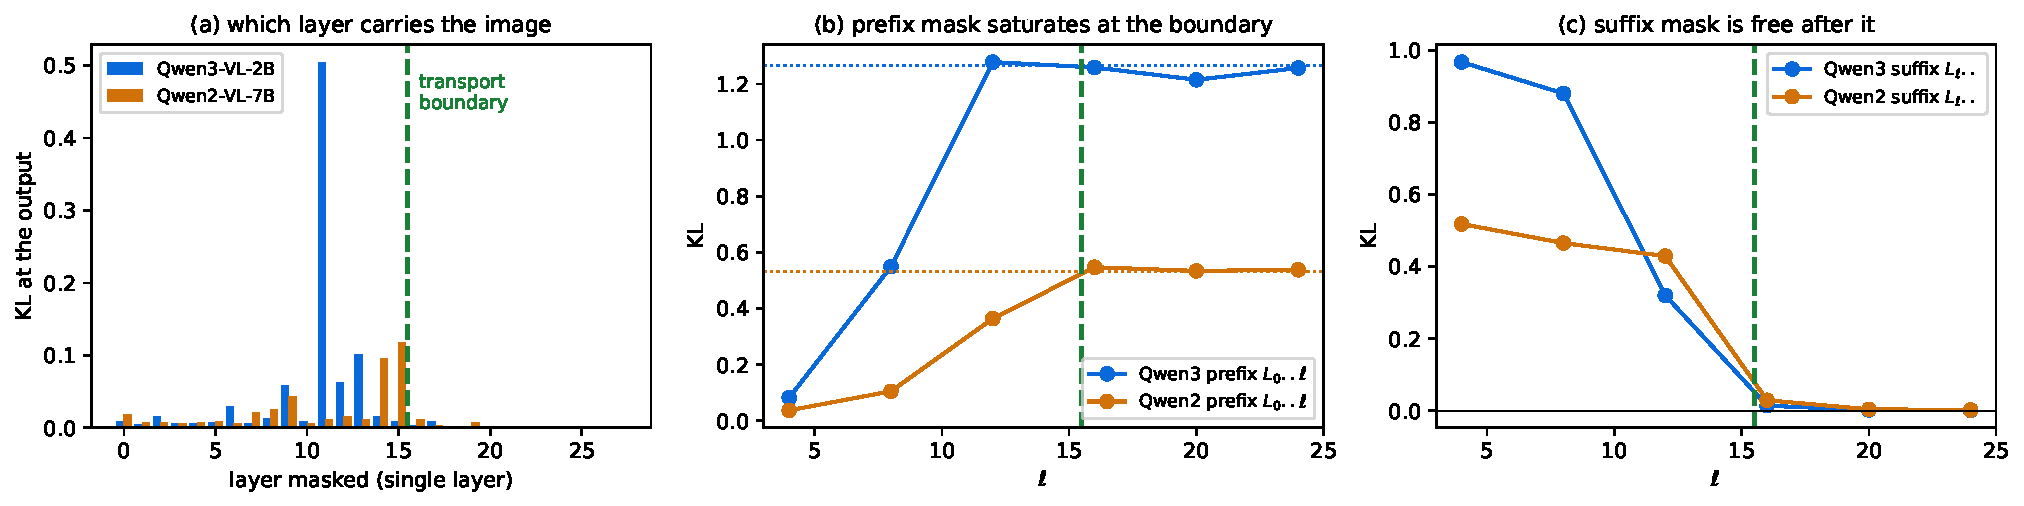
\includegraphics[width=\textwidth]{figs/fig_transport.pdf}
\caption{\textbf{The transport measurement.} (a) Masking one layer's image attention at a time: the effect is
concentrated well before the boundary and is at or below $0.0023$ from L20 on both models. (b) Masking a prefix
$L_0..\ell$ reaches the full-mask value (dotted) once $\ell$ passes the window. (c) Masking a suffix
$L_\ell..\text{end}$ costs nothing once $\ell$ is past it. Three readings, one boundary.}
\label{fig:transport}
\end{figure}

Single-layer masks peak at L11 on Qwen3 (KL $0.504$; next highest L13 at $0.101$) and at L15/L14 on Qwen2
($0.118$/$0.096$). From L20 onward every layer is at or below $0.0023$ on both models. On Qwen3-VL-8B, which has
$36$ layers, the same behaviour appears at L21, i.e.\ the same $0.57$ fraction of depth.

\paragraph{Three independent readings of the same boundary.} The masks are one. Pruning is the second: discarding
$90\%$ of visual tokens at the boundary costs $+0.0$ to $+0.5$ points across ten stratum-cells, whereas moving the
same cut to $\ell{=}4$ costs $5.2$ more on one model ($0.5$ on the other), and a taper that removes half the tokens
at $\ell{=}9$--$12$ loses $3.5$ points against not pruning at matched tokens while buying nothing over a single cut
($-1.0$). Read-out depth is the third: restricting the localiser to layers $\le$ L20 costs $-0.5$ and $+1.6$ points
of coverage, while restricting it to $\le$ L16 costs $9.4$ and $22.0$. Transport finishes at the boundary; the
signal the ranking reads is produced after it.

\section{Depth structure across checkpoints}\label{app:depth}

\begin{table}[h]\centering\small
\caption{Where each quantity falls, per checkpoint. The transport boundary and the read-out band are fractions of
depth, not fixed layer indices, which is what lets both policies transfer to a $36$-layer model unchanged. The
$36$-layer boundary is masked: its suffix is harmless at L20 and zero from L24, the same fractions as the pair.}
\begin{tabular}{lccccc}
\toprule
checkpoint & layers & block-mean band & read-out band & boundary & boundary / depth\\
\midrule
Qwen3-VL-2B & 28 & L16--L26 & L17--L20 & L16 & 0.57\\
Qwen2-VL-7B & 28 & L15--L26 & L19--L22 & L16 & 0.57\\
Qwen2.5-VL-7B & 28 & L16--L26 & --- & L16 & 0.57\\
Qwen3-VL-8B & \textbf{36} & L20--L33 & --- & \textbf{L21} & 0.57\\
\bottomrule
\end{tabular}\label{tab:depth}
\end{table}

\section{Mechanism: three stages, three interventions}\label{app:mech}

\begin{figure}[h]\centering
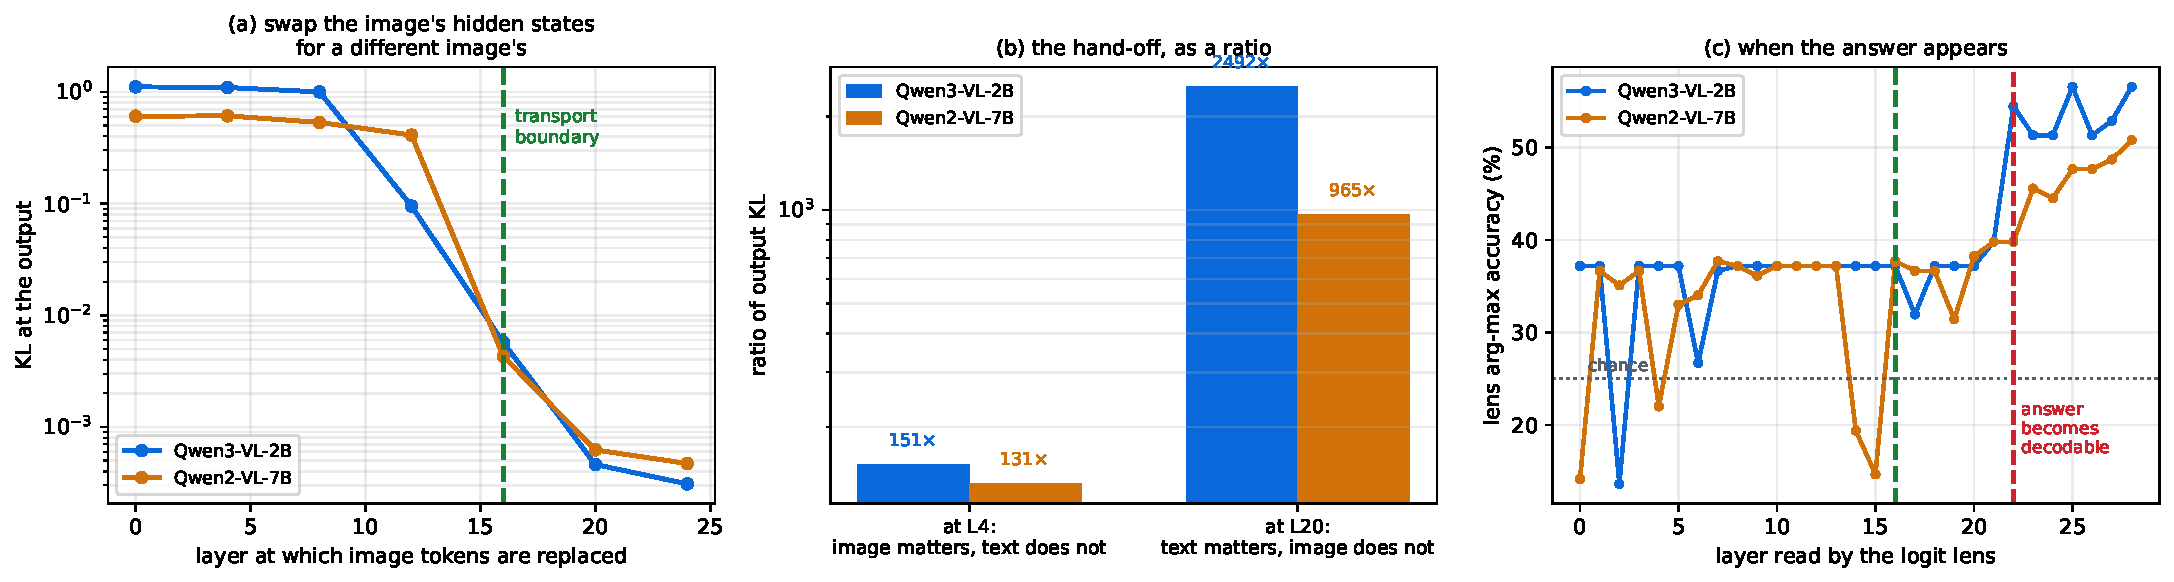
\includegraphics[width=\textwidth]{figs/fig_mechanism.pdf}
\caption{\textbf{(a)} Replacing the image tokens' hidden states at layer $\ell$ with a different image's: the
output effect falls three orders of magnitude across the boundary. \textbf{(b)} The hand-off as a ratio: early,
the image dominates and the text is inert; late, exactly the reverse. \textbf{(c)} Logit lens at the answer
position: the correct option becomes decodable only in the last quarter of the stack.}
\label{fig:mech}
\end{figure}

Each row of Table~\ref{tab:stages} is measured by a different intervention, so no stage rests on the method that
found another.

\begin{table}[h]\centering\small
\caption{The three stages. Every number is measured on both core checkpoints.}
\setlength{\tabcolsep}{4pt}\begin{tabular}{p{2.2cm}p{1.35cm}p{2.8cm}p{5.5cm}}
\toprule
stage & layers & measured by & evidence\\
\midrule
image $\to$ text transport & L0--L16 & attention masking; hidden-state patching & suffix masks cost nothing from L16 ($0.014$, $0.029$); the patch effect falls $17\times$ and $96\times$ between L12 and L16\\
question-conditioned read-out & L17--L21 & end-task accuracy by read-out depth & crop accuracy spans $34.6$--$70.2$, peaking at L17; no layer inside the window beats not cropping\\
answer formation & L22+ & logit lens & lens accuracy steps $+18.0$ [$+8.7,+27.0$] and $+14.2$ [$+7.2,+21.3$] above its early plateau\\
\bottomrule
\end{tabular}\label{tab:stages}
\end{table}

The logit lens is computed with the final norm applied to intermediate layers only; applying it to the last hidden
state as well double-normalises and corrupts that layer alone, which cost us a retracted result earlier in this
project. We assert per run that our last-layer read-out matches the true logits.

A fourth, independent technique places the read-out band in the same spot: a ridge probe from the
answer-position state to the target's location rises across the transport window and peaks at L18--19 (Qwen3,
$r=+0.635$) and L18 (Qwen2, $+0.603$).

\paragraph{The channel and the values.} Masking blocks the text$\to$image attention \emph{channel}; it does not
show that the image information is absent from the residual stream. Replacing the image tokens' hidden states
with a donor image's (same question, same token budget) closes that gap. The effect falls three orders of
magnitude across the boundary, and both pre-registered controls behave as required: patching the image at L4 is
large, patching text at L20 is large.

\begin{table}[t]
\caption{Representation patching: replace the image tokens' hidden states at one layer's output with a donor
image's; KL at the output and answer flips. Text controls patch text-token states at the same depth.}
\label{tab:patch}
\begin{center}
\small
\begin{tabular}{lcc}
\multicolumn{1}{c}{\bf patch site} &\multicolumn{1}{c}{\bf Qwen3-VL-2B KL (flips)} &\multicolumn{1}{c}{\bf Qwen2-VL-7B KL (flips)}
\\ \hline \\
image L0 & 1.758 (61.7\%) & 0.800 (60.0\%)\\
image L4 (control C1) & 1.766 (63.3\%) & 0.798 (58.3\%)\\
image L8 & 1.622 (60.0\%) & 0.657 (60.0\%)\\
image L12 & 0.134 (16.7\%) & 0.517 (51.7\%)\\
image L16 & 0.009 (3.3\%) & 0.005 (5.0\%)\\
image L20 & 0.0005 (0\%) & 0.0008 (1.7\%)\\
image L24 & 0.0003 (0\%) & 0.0006 (1.7\%)\\
text L4 & 0.009 (5.0\%) & 0.006 (3.3\%)\\
text L20 (control C2) & 1.834 (63.3\%) & 0.802 (60.0\%)\\
\end{tabular}
\end{center}
\end{table}

The late-image arm lands exactly on the text-L4 noise floor ($0.009$ vs $0.009$ on Qwen3; $0.005$ vs $0.006$ on
Qwen2), and the two controls invert cleanly across depth: at L4 the image matters $151\times$/$131\times$ more
than the text, at L20 the text matters $2492\times$/$965\times$ more than the image. Two different
interventions, two checkpoints, one boundary.

\paragraph{The boundary at the AVR operating point.} AVR encodes at $900$ tokens and prunes at the boundary, so
inertness must hold on the unpruned $900$-token pass. Injecting donor values at the layer's output:

\begin{table}[t]
\caption{Value inertness at $900$ tokens (Qwen3-VL-2B, $n=191$): donor hidden states at the layer's output.}
\label{tab:inert900}
\begin{center}
\small
\begin{tabular}{lcc}
\multicolumn{1}{c}{\bf patch at 900 tokens} &\multicolumn{1}{c}{\bf mean KL} &\multicolumn{1}{c}{\bf answer flips}
\\ \hline \\
dropped positions @L16 (810 of 900) & 0.0022 & 1.0\%\\
kept positions @L16 (90 of 900) & 0.0065 & 3.1\%\\
dropped positions @L8 (transport window) & 0.3407 & 20.9\%\\
\end{tabular}
\end{center}
\end{table}

At the boundary the values are inert whether or not they are the ones AVR keeps; inside the transport window
the same intervention moves one answer in five.

\paragraph{The cost of misplacing the boundary.} Pruning is free at the boundary and expensive before it. With
the same number of tokens dropped and a large negative attention bias on the dropped columns from layer $K$
onward (functionally FastV's rule):

\begin{table}[t]
\caption{Pruning depth and selection. V*Bench, $n=191$; every arm prunes the same count.}
\label{tab:prunedepth}
\begin{center}
\small
\begin{tabular}{lccc}
\multicolumn{1}{c}{\bf keep} &\multicolumn{1}{c}{\bf random} &\multicolumn{1}{c}{\bf layer-2 (FastV default)} &\multicolumn{1}{c}{\bf late read-out (L16--26)}
\\ \hline \\
10\% & 38.2\% & 34.6\% & 56.0\%\\
25\% & 41.4\% & 40.3\% & 58.1\%\\
50\% & 47.1\% & 52.9\% & 55.5\%\\
\end{tabular}
\end{center}
\end{table}

No pruning is $56.5\%$. Ranking at layer 2 costs $22.0$ points against no pruning and is $3.7$ points
\emph{worse than random}; the late read-out deletes $90\%$ of visual tokens at $-0.5$ points [$-5.8,+4.7$] and
the learned criterion at $+2.1$ [$-2.6,+6.8$]. The collapse replicates on Qwen2-VL-7B (late over layer-2
$+11.5$ [$+4.2,+18.8$] at $10\%$ keep; layer-2 is $4.7$ points below random) and is larger on general VQA:
layer-2 against random is $-15.0$ [$-22.0,-7.5$] on POPE and $-25.5$ [$-33.0,-18.0$] on MMBench.

\paragraph{Selection stops mattering at the boundary.} Before the boundary, which tokens survive matters: a
layer-4 probe beats random keep by $+8.4$ [$+2.1,+15.2$] and $+8.9$ [$+2.6,+15.2$] at $25\%$ keep. At and after
it, the choice is irrelevant: random keep matches attention keep on both models at every keep ratio tested,
and pruning is free ($0.0$--$0.5$ points in $9$ of $10$ cells). The boundary is not merely where pruning
becomes cheap; it is where selection ceases to matter.

\section{Late-depth behaviour: agnosticism, merging, and disagreement}\label{app:late}

\paragraph{The late layers are agnostic to the image.} Three independent probes agree that direct image access stops
mattering at the boundary: the suffix mask, the image-value patch, and the answer-row-only mask. The suffix mask is
the same intervention as the boundary measurement; the value patch replaces the image tokens' hidden states with a
donor image's; the answer-row mask blocks only the final prompt position's image access at every layer.


\paragraph{Image and text tokens merge in the late stack.} The patching controls invert across depth: early, the image
values dominate and the text values are inert; late, exactly the reverse. Replacing image values past the boundary
lands on the irrelevant-text noise floor, so the image tokens behave like ordinary, interchangeable context tokens
whose information has already been absorbed into the text stream. The answer position confirms the direction of the
hand-off: it cannot read the image directly, and the evidence arrives through the text representations that
consolidated it.

\begin{table}[t]
\caption{The hand-off. Donor patching at L4 and L20, both checkpoints; ratios compare the two patch sites. Paired
KL difference between the L16 and L4 image patches is $-1.757$ [$-2.308,-1.256$] and $-0.792$ [$-1.031,-0.577$].}
\label{tab:handoff}
\begin{center}
\small
\begin{tabular}{lcccc}
\multicolumn{1}{c}{\bf site} &\multicolumn{1}{c}{\bf image patch (Q3/Q2)} &\multicolumn{1}{c}{\bf text patch (Q3/Q2)} &\multicolumn{1}{c}{\bf ratio}
\\ \hline \\
L4 & 1.766 / 0.798 & 0.009 / 0.006 & image $151\times$ / $131\times$\\
L20 & 0.0005 / 0.0008 & 1.834 / 0.802 & text $2492\times$ / $965\times$\\
\end{tabular}
\end{center}
\end{table}

\paragraph{The layers disagree about where to look.} The 28 layer maps are not variations on one map. Mean off-diagonal
arg-max agreement across the $28\times28$ layer pairs is $13.8\%$/$38.1\%$, and the agreement matrix has block
structure that splits at the transport boundary. The usable placement signal exists only after it.


Consequently, every label-free layer-disagreement rule from the language-model literature was ported to the
read-out and compared with the fixed gate; none beats it, and most lose badly.

\begin{table}[t]
\caption{Label-free layer-selection rules, coverage@$0.25$ minus the fixed gate, four architectures.}
\label{tab:rules}
\begin{center}
\small
\begin{tabular}{lcccc}
\multicolumn{1}{c}{\bf rule} &\multicolumn{1}{c}{\bf Qwen3} &\multicolumn{1}{c}{\bf Qwen2} &\multicolumn{1}{c}{\bf LLaVA-NeXT} &\multicolumn{1}{c}{\bf OneVision}
\\ \hline \\
gate max (reference, coverage \%) & 56.0 & 51.8 & 25.7 & 23.6\\
CLD entropy-valley layer & $-12.0$ & $-1.0$ & $+0.5$ & $+4.2$\\
attention-entropy-min layer & $-2.6$ & $+2.1$ & $+0.0$ & $+1.0$\\
attention-JSD vs final & $+1.0$ & $-1.0$ & $+1.6$ & $-10.5$\\
ASL rank-stability layer & $-11.5$ & $-8.4$ & $+0.0$ & $-6.8$\\
depth-EMA of ranks & $-13.6$ & $-6.8$ & $+0.5$ & $+2.1$\\
SLED extrapolation & $+0.5$ & $-0.5$ & $+2.1$ & $+2.1$\\
\end{tabular}
\end{center}
\end{table}

.

\section{The transport measurement in full}\label{app:transport}

A forward pre-hook on every decoder layer adds $-10^4$ to the attention logits of chosen query rows over the
image-token columns, at chosen layers only. Masking \emph{all} text rows at \emph{all} layers destroys the answer
(KL $1.266$ / $0.532$, $42\%$ / $45\%$ of answers flip, $n{=}40$); masking only the answer token's row at all layers
does not (KL $0.025$, $3\%$ flip). Table~\ref{tab:prefix} localises the window.


\begin{figure}[h]\centering
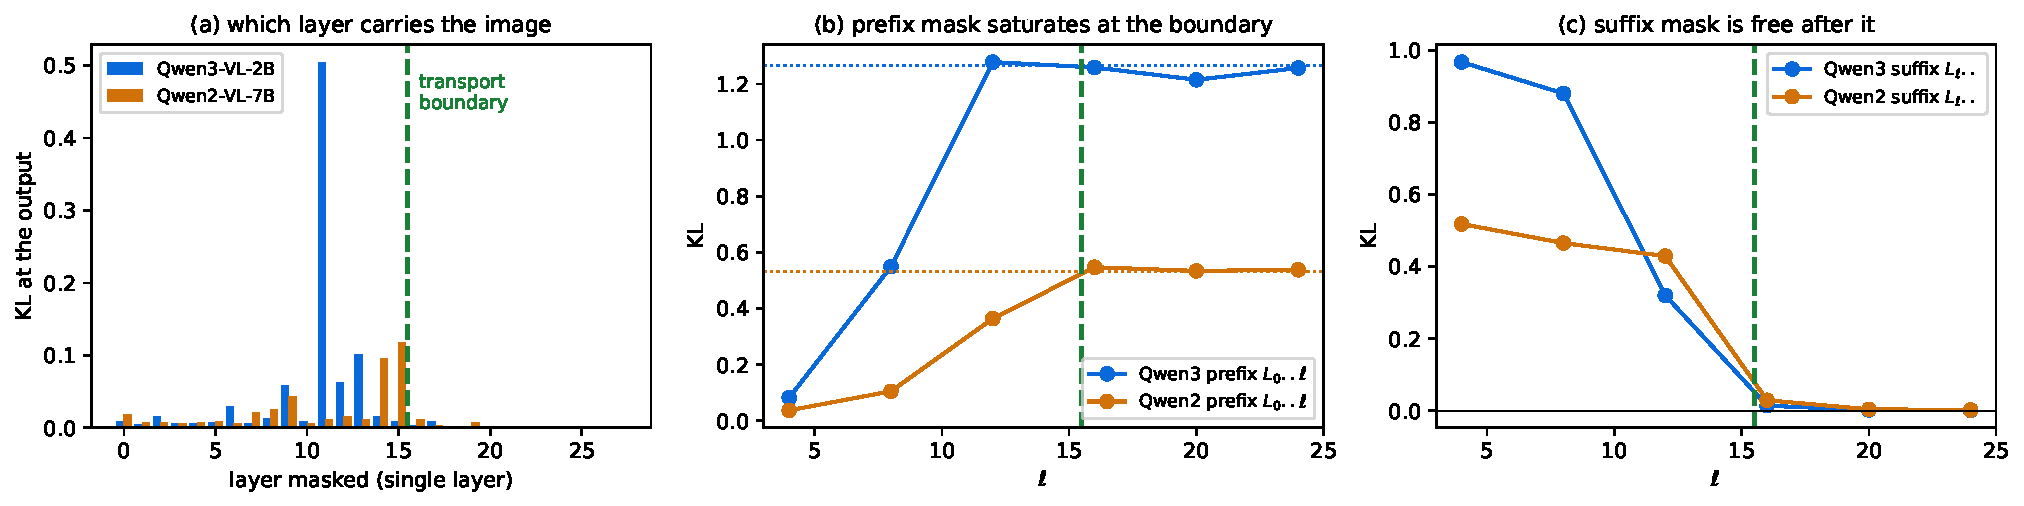
\includegraphics[width=\textwidth]{figs/fig_transport.pdf}
\caption{\textbf{The transport measurement.} (a) Masking one layer's image attention at a time: the effect is
concentrated well before the boundary and is at or below $0.0023$ from L20 on both models. (b) Masking a prefix
$L_0..\ell$ reaches the full-mask value (dotted) once $\ell$ passes the window. (c) Masking a suffix
$L_\ell..\text{end}$ costs nothing once $\ell$ is past it. Three readings, one boundary.}
\label{fig:transport}
\end{figure}

Single-layer masks peak at L11 on Qwen3 (KL $0.504$; next highest L13 at $0.101$) and at L15/L14 on Qwen2
($0.118$/$0.096$). From L20 onward every layer is at or below $0.0023$ on both models. On Qwen3-VL-8B, which has
$36$ layers, the same behaviour appears at L21, i.e.\ the same $0.57$ fraction of depth.

\paragraph{Three independent readings of the same boundary.} The masks are one. Pruning is the second: discarding
$90\%$ of visual tokens at the boundary costs $+0.0$ to $+0.5$ points across ten stratum-cells, whereas moving the
same cut to $\ell{=}4$ costs $5.2$ more on one model ($0.5$ on the other), and a taper that removes half the tokens
at $\ell{=}9$--$12$ loses $3.5$ points against not pruning at matched tokens while buying nothing over a single cut
($-1.0$). Read-out depth is the third: restricting the localiser to layers $\le$ L20 costs $-0.5$ and $+1.6$ points
of coverage, while restricting it to $\le$ L16 costs $9.4$ and $22.0$. Transport finishes at the boundary; the
signal the ranking reads is produced after it.

\section{Depth structure across checkpoints}\label{app:depth}

\begin{table}[h]\centering\small
\caption{Where each quantity falls, per checkpoint. The transport boundary and the read-out band are fractions of
depth, not fixed layer indices, which is what lets both policies transfer to a $36$-layer model unchanged. The
$36$-layer boundary is masked: its suffix is harmless at L20 and zero from L24, the same fractions as the pair.}
\begin{tabular}{lccccc}
\toprule
checkpoint & layers & block-mean band & read-out band & boundary & boundary / depth\\
\midrule
Qwen3-VL-2B & 28 & L16--L26 & L17--L20 & L16 & 0.57\\
Qwen2-VL-7B & 28 & L15--L26 & L19--L22 & L16 & 0.57\\
Qwen2.5-VL-7B & 28 & L16--L26 & --- & L16 & 0.57\\
Qwen3-VL-8B & \textbf{36} & L20--L33 & --- & \textbf{L21} & 0.57\\
\bottomrule
\end{tabular}\label{tab:depth}
\end{table}

\section{Mechanism: three stages, three interventions}\label{app:mech}

\begin{figure}[h]\centering
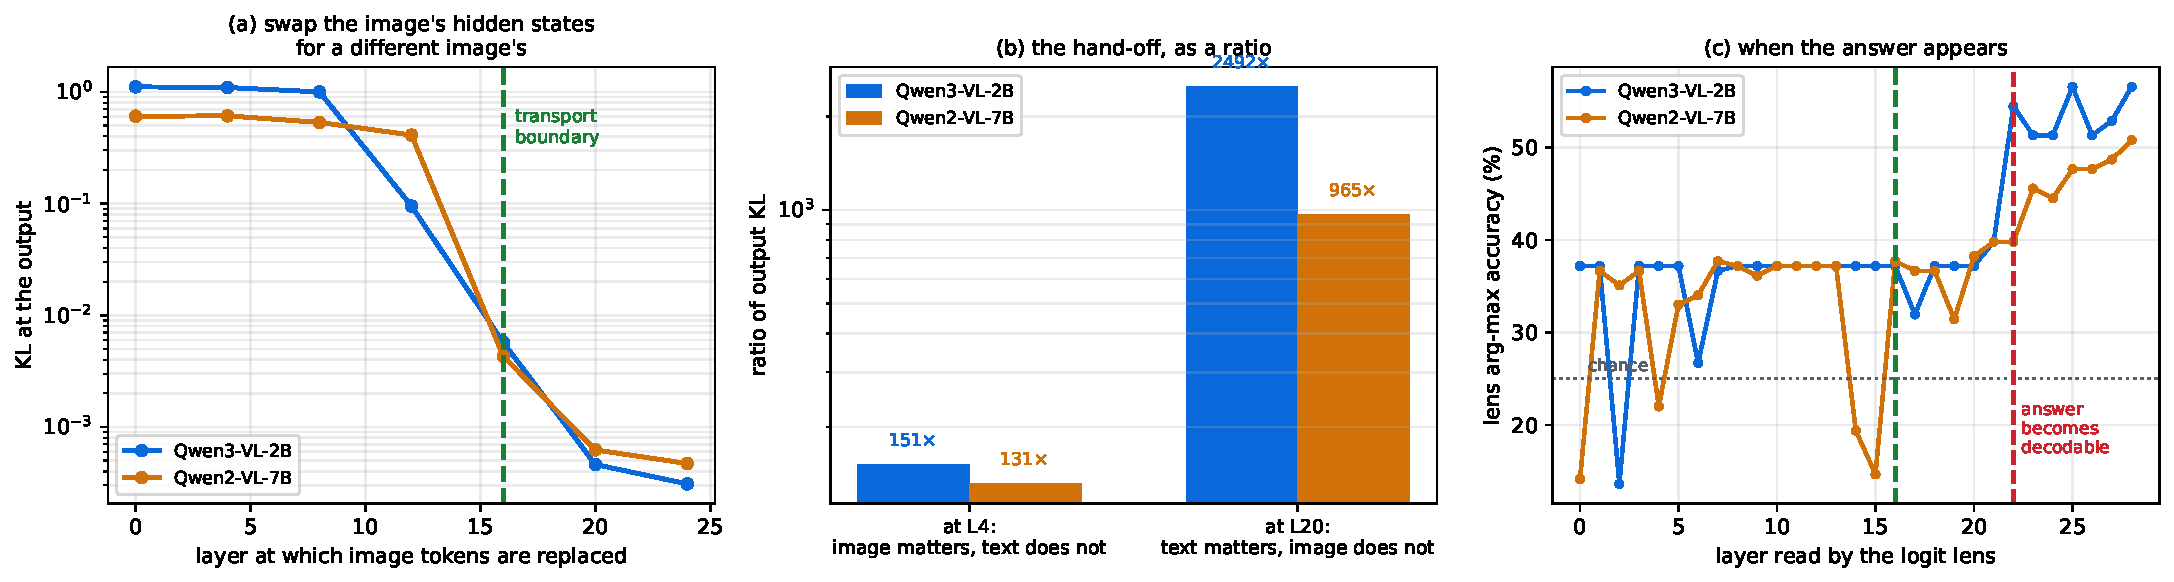
\includegraphics[width=\textwidth]{figs/fig_mechanism.pdf}
\caption{\textbf{(a)} Replacing the image tokens' hidden states at layer $\ell$ with a different image's: the
output effect falls three orders of magnitude across the boundary. \textbf{(b)} The hand-off as a ratio: early,
the image dominates and the text is inert; late, exactly the reverse. \textbf{(c)} Logit lens at the answer
position: the correct option becomes decodable only in the last quarter of the stack.}
\label{fig:mech}
\end{figure}

Each row of Table~\ref{tab:stages} is measured by a different intervention, so no stage rests on the method that
found another.

\begin{table}[h]\centering\small
\caption{The three stages. Every number is measured on both core checkpoints.}
\setlength{\tabcolsep}{4pt}\begin{tabular}{p{2.2cm}p{1.35cm}p{2.8cm}p{5.5cm}}
\toprule
stage & layers & measured by & evidence\\
\midrule
image $\to$ text transport & L0--L16 & attention masking; hidden-state patching & suffix masks cost nothing from L16 ($0.014$, $0.029$); the patch effect falls $17\times$ and $96\times$ between L12 and L16\\
question-conditioned read-out & L17--L21 & end-task accuracy by read-out depth & crop accuracy spans $34.6$--$70.2$, peaking at L17; no layer inside the window beats not cropping\\
answer formation & L22+ & logit lens & lens accuracy steps $+18.0$ [$+8.7,+27.0$] and $+14.2$ [$+7.2,+21.3$] above its early plateau\\
\bottomrule
\end{tabular}\label{tab:stages}
\end{table}

The logit lens is computed with the final norm applied to intermediate layers only; applying it to the last hidden
state as well double-normalises and corrupts that layer alone, which cost us a retracted result earlier in this
project. We assert per run that our last-layer read-out matches the true logits.

A fourth, independent technique places the read-out band in the same spot: a ridge probe from the
answer-position state to the target's location rises across the transport window and peaks at L18--19 (Qwen3,
$r=+0.635$) and L18 (Qwen2, $+0.603$).

\paragraph{The channel and the values.} Masking blocks the text$\to$image attention \emph{channel}; it does not
show that the image information is absent from the residual stream. Replacing the image tokens' hidden states
with a donor image's (same question, same token budget) closes that gap. The effect falls three orders of
magnitude across the boundary, and both pre-registered controls behave as required: patching the image at L4 is
large, patching text at L20 is large.

\begin{table}[t]
\caption{Representation patching: replace the image tokens' hidden states at one layer's output with a donor
image's; KL at the output and answer flips. Text controls patch text-token states at the same depth.}
\label{tab:patch}
\begin{center}
\small
\begin{tabular}{lcc}
\multicolumn{1}{c}{\bf patch site} &\multicolumn{1}{c}{\bf Qwen3-VL-2B KL (flips)} &\multicolumn{1}{c}{\bf Qwen2-VL-7B KL (flips)}
\\ \hline \\
image L0 & 1.758 (61.7\%) & 0.800 (60.0\%)\\
image L4 (control C1) & 1.766 (63.3\%) & 0.798 (58.3\%)\\
image L8 & 1.622 (60.0\%) & 0.657 (60.0\%)\\
image L12 & 0.134 (16.7\%) & 0.517 (51.7\%)\\
image L16 & 0.009 (3.3\%) & 0.005 (5.0\%)\\
image L20 & 0.0005 (0\%) & 0.0008 (1.7\%)\\
image L24 & 0.0003 (0\%) & 0.0006 (1.7\%)\\
text L4 & 0.009 (5.0\%) & 0.006 (3.3\%)\\
text L20 (control C2) & 1.834 (63.3\%) & 0.802 (60.0\%)\\
\end{tabular}
\end{center}
\end{table}

The late-image arm lands exactly on the text-L4 noise floor ($0.009$ vs $0.009$ on Qwen3; $0.005$ vs $0.006$ on
Qwen2), and the two controls invert cleanly across depth: at L4 the image matters $151\times$/$131\times$ more
than the text, at L20 the text matters $2492\times$/$965\times$ more than the image. Two different
interventions, two checkpoints, one boundary.

\paragraph{The boundary at the AVR operating point.} AVR encodes at $900$ tokens and prunes at the boundary, so
inertness must hold on the unpruned $900$-token pass. Injecting donor values at the layer's output:

\begin{table}[t]
\caption{Value inertness at $900$ tokens (Qwen3-VL-2B, $n=191$): donor hidden states at the layer's output.}
\label{tab:inert900}
\begin{center}
\small
\begin{tabular}{lcc}
\multicolumn{1}{c}{\bf patch at 900 tokens} &\multicolumn{1}{c}{\bf mean KL} &\multicolumn{1}{c}{\bf answer flips}
\\ \hline \\
dropped positions @L16 (810 of 900) & 0.0022 & 1.0\%\\
kept positions @L16 (90 of 900) & 0.0065 & 3.1\%\\
dropped positions @L8 (transport window) & 0.3407 & 20.9\%\\
\end{tabular}
\end{center}
\end{table}

At the boundary the values are inert whether or not they are the ones AVR keeps; inside the transport window
the same intervention moves one answer in five.

\paragraph{The cost of misplacing the boundary.} Pruning is free at the boundary and expensive before it. With
the same number of tokens dropped and a large negative attention bias on the dropped columns from layer $K$
onward (functionally FastV's rule):

\begin{table}[t]
\caption{Pruning depth and selection. V*Bench, $n=191$; every arm prunes the same count.}
\label{tab:prunedepth}
\begin{center}
\small
\begin{tabular}{lccc}
\multicolumn{1}{c}{\bf keep} &\multicolumn{1}{c}{\bf random} &\multicolumn{1}{c}{\bf layer-2 (FastV default)} &\multicolumn{1}{c}{\bf late read-out (L16--26)}
\\ \hline \\
10\% & 38.2\% & 34.6\% & 56.0\%\\
25\% & 41.4\% & 40.3\% & 58.1\%\\
50\% & 47.1\% & 52.9\% & 55.5\%\\
\end{tabular}
\end{center}
\end{table}

No pruning is $56.5\%$. Ranking at layer 2 costs $22.0$ points against no pruning and is $3.7$ points
\emph{worse than random}; the late read-out deletes $90\%$ of visual tokens at $-0.5$ points [$-5.8,+4.7$] and
the learned criterion at $+2.1$ [$-2.6,+6.8$]. The collapse replicates on Qwen2-VL-7B (late over layer-2
$+11.5$ [$+4.2,+18.8$] at $10\%$ keep; layer-2 is $4.7$ points below random) and is larger on general VQA:
layer-2 against random is $-15.0$ [$-22.0,-7.5$] on POPE and $-25.5$ [$-33.0,-18.0$] on MMBench.

\paragraph{Selection stops mattering at the boundary.} Before the boundary, which tokens survive matters: a
layer-4 probe beats random keep by $+8.4$ [$+2.1,+15.2$] and $+8.9$ [$+2.6,+15.2$] at $25\%$ keep. At and after
it, the choice is irrelevant: random keep matches attention keep on both models at every keep ratio tested,
and pruning is free ($0.0$--$0.5$ points in $9$ of $10$ cells). The boundary is not merely where pruning
becomes cheap; it is where selection ceases to matter.

\section{Late-depth behaviour: agnosticism, merging, and disagreement}\label{app:late}

\paragraph{The late layers are agnostic to the image.} Three independent probes agree that direct image access stops
mattering at the boundary: the suffix mask, the image-value patch, and the answer-row-only mask. The suffix mask is
the same intervention as the boundary measurement; the value patch replaces the image tokens' hidden states with a
donor image's; the answer-row mask blocks only the final prompt position's image access at every layer.


\paragraph{Image and text tokens merge in the late stack.} The patching controls invert across depth: early, the image
values dominate and the text values are inert; late, exactly the reverse. Replacing image values past the boundary
lands on the irrelevant-text noise floor, so the image tokens behave like ordinary, interchangeable context tokens
whose information has already been absorbed into the text stream. The answer position confirms the direction of the
hand-off: it cannot read the image directly, and the evidence arrives through the text representations that
consolidated it.

\begin{table}[t]
\caption{The hand-off. Donor patching at L4 and L20, both checkpoints; ratios compare the two patch sites. Paired
KL difference between the L16 and L4 image patches is $-1.757$ [$-2.308,-1.256$] and $-0.792$ [$-1.031,-0.577$].}
\label{tab:handoff}
\begin{center}
\small
\begin{tabular}{lcccc}
\multicolumn{1}{c}{\bf site} &\multicolumn{1}{c}{\bf image patch (Q3/Q2)} &\multicolumn{1}{c}{\bf text patch (Q3/Q2)} &\multicolumn{1}{c}{\bf ratio}
\\ \hline \\
L4 & 1.766 / 0.798 & 0.009 / 0.006 & image $151\times$ / $131\times$\\
L20 & 0.0005 / 0.0008 & 1.834 / 0.802 & text $2492\times$ / $965\times$\\
\end{tabular}
\end{center}
\end{table}

\paragraph{The layers disagree about where to look.} The 28 layer maps are not variations on one map. Mean off-diagonal
arg-max agreement across the $28\times28$ layer pairs is $13.8\%$/$38.1\%$, and the agreement matrix has block
structure that splits at the transport boundary. The usable placement signal exists only after it.


Consequently, every label-free layer-disagreement rule from the language-model literature was ported to the
read-out and compared with the fixed gate; none beats it, and most lose badly.

\begin{table}[t]
\caption{Label-free layer-selection rules, coverage@$0.25$ minus the fixed gate, four architectures.}
\label{tab:rules}
\begin{center}
\small
\begin{tabular}{lcccc}
\multicolumn{1}{c}{\bf rule} &\multicolumn{1}{c}{\bf Qwen3} &\multicolumn{1}{c}{\bf Qwen2} &\multicolumn{1}{c}{\bf LLaVA-NeXT} &\multicolumn{1}{c}{\bf OneVision}
\\ \hline \\
gate max (reference, coverage \%) & 56.0 & 51.8 & 25.7 & 23.6\\
CLD entropy-valley layer & $-12.0$ & $-1.0$ & $+0.5$ & $+4.2$\\
attention-entropy-min layer & $-2.6$ & $+2.1$ & $+0.0$ & $+1.0$\\
attention-JSD vs final & $+1.0$ & $-1.0$ & $+1.6$ & $-10.5$\\
ASL rank-stability layer & $-11.5$ & $-8.4$ & $+0.0$ & $-6.8$\\
depth-EMA of ranks & $-13.6$ & $-6.8$ & $+0.5$ & $+2.1$\\
SLED extrapolation & $+0.5$ & $-0.5$ & $+2.1$ & $+2.1$\\
\end{tabular}
\end{center}
\end{table}

.

\section{The transport measurement in full}\label{app:transport}

A forward pre-hook on every decoder layer adds $-10^4$ to the attention logits of chosen query rows over the
image-token columns, at chosen layers only. Masking \emph{all} text rows at \emph{all} layers destroys the answer
(KL $1.266$ / $0.532$, $42\%$ / $45\%$ of answers flip, $n{=}40$); masking only the answer token's row at all layers
does not (KL $0.025$, $3\%$ flip). Table~\ref{tab:prefix} localises the window.


\begin{figure}[h]\centering
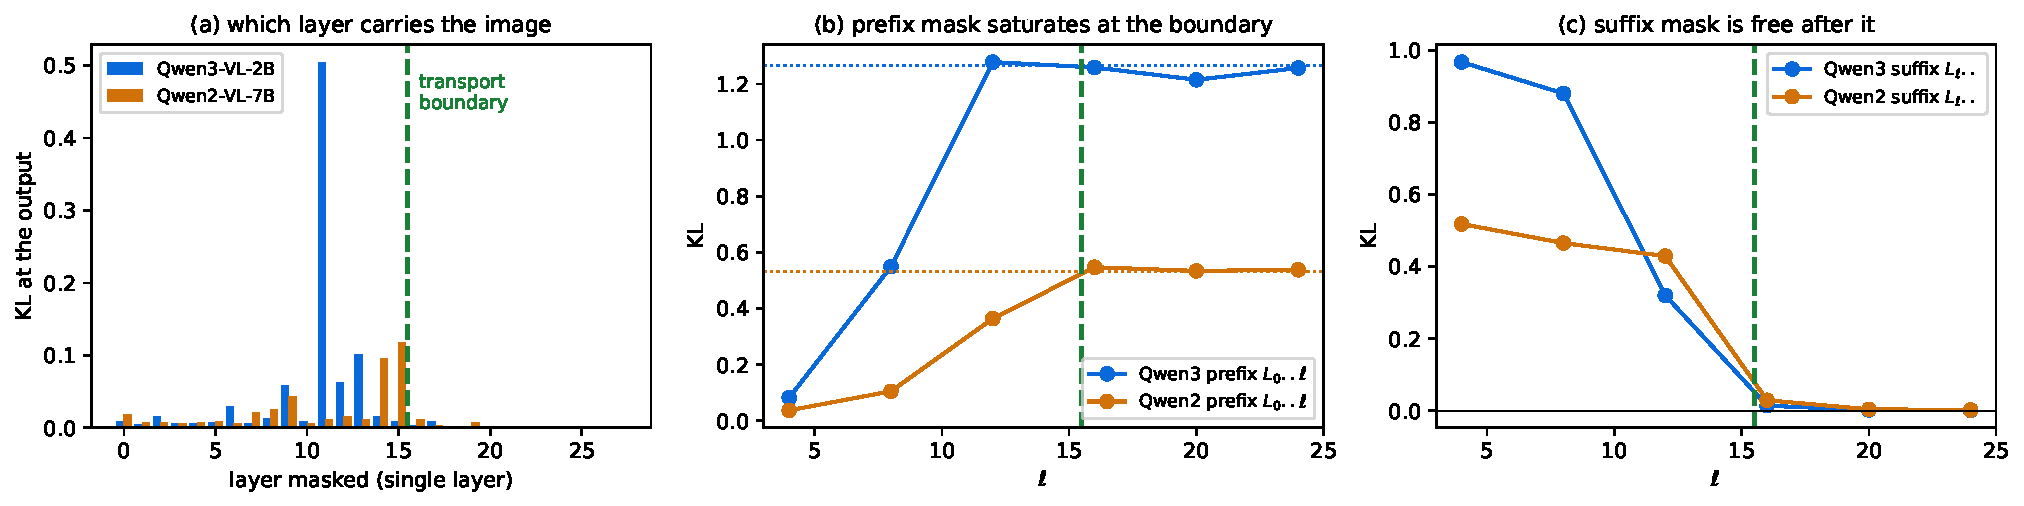
\includegraphics[width=\textwidth]{figs/fig_transport.pdf}
\caption{\textbf{The transport measurement.} (a) Masking one layer's image attention at a time: the effect is
concentrated well before the boundary and is at or below $0.0023$ from L20 on both models. (b) Masking a prefix
$L_0..\ell$ reaches the full-mask value (dotted) once $\ell$ passes the window. (c) Masking a suffix
$L_\ell..\text{end}$ costs nothing once $\ell$ is past it. Three readings, one boundary.}
\label{fig:transport}
\end{figure}

Single-layer masks peak at L11 on Qwen3 (KL $0.504$; next highest L13 at $0.101$) and at L15/L14 on Qwen2
($0.118$/$0.096$). From L20 onward every layer is at or below $0.0023$ on both models. On Qwen3-VL-8B, which has
$36$ layers, the same behaviour appears at L21, i.e.\ the same $0.57$ fraction of depth.

\paragraph{Three independent readings of the same boundary.} The masks are one. Pruning is the second: discarding
$90\%$ of visual tokens at the boundary costs $+0.0$ to $+0.5$ points across ten stratum-cells, whereas moving the
same cut to $\ell{=}4$ costs $5.2$ more on one model ($0.5$ on the other), and a taper that removes half the tokens
at $\ell{=}9$--$12$ loses $3.5$ points against not pruning at matched tokens while buying nothing over a single cut
($-1.0$). Read-out depth is the third: restricting the localiser to layers $\le$ L20 costs $-0.5$ and $+1.6$ points
of coverage, while restricting it to $\le$ L16 costs $9.4$ and $22.0$. Transport finishes at the boundary; the
signal the ranking reads is produced after it.

\section{Depth structure across checkpoints}\label{app:depth}

\begin{table}[h]\centering\small
\caption{Where each quantity falls, per checkpoint. The transport boundary and the read-out band are fractions of
depth, not fixed layer indices, which is what lets both policies transfer to a $36$-layer model unchanged. The
$36$-layer boundary is masked: its suffix is harmless at L20 and zero from L24, the same fractions as the pair.}
\begin{tabular}{lccccc}
\toprule
checkpoint & layers & block-mean band & read-out band & boundary & boundary / depth\\
\midrule
Qwen3-VL-2B & 28 & L16--L26 & L17--L20 & L16 & 0.57\\
Qwen2-VL-7B & 28 & L15--L26 & L19--L22 & L16 & 0.57\\
Qwen2.5-VL-7B & 28 & L16--L26 & --- & L16 & 0.57\\
Qwen3-VL-8B & \textbf{36} & L20--L33 & --- & \textbf{L21} & 0.57\\
\bottomrule
\end{tabular}\label{tab:depth}
\end{table}

\section{Mechanism: three stages, three interventions}\label{app:mech}

\begin{figure}[h]\centering
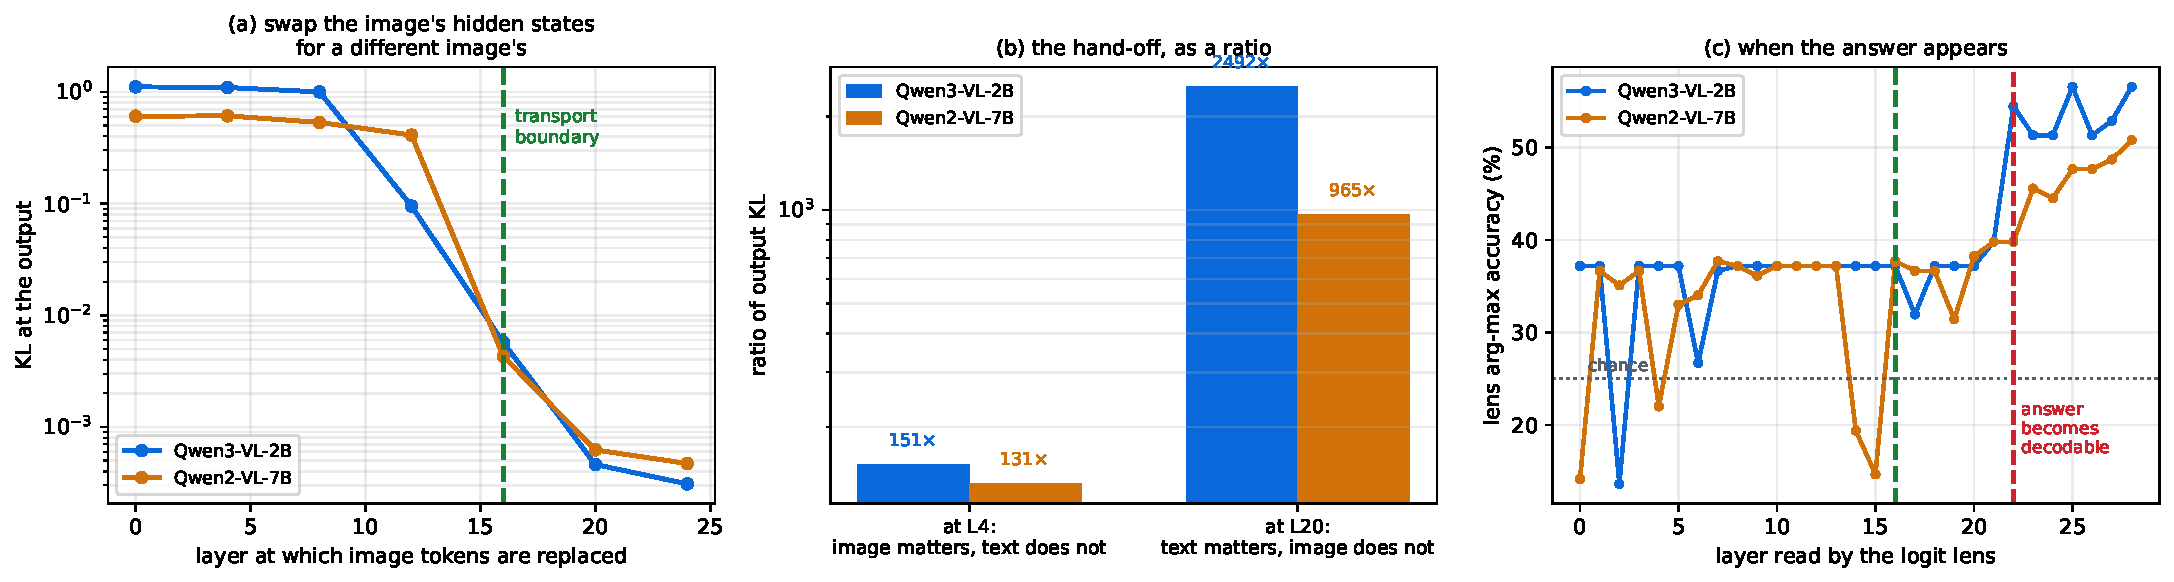
\includegraphics[width=\textwidth]{figs/fig_mechanism.pdf}
\caption{\textbf{(a)} Replacing the image tokens' hidden states at layer $\ell$ with a different image's: the
output effect falls three orders of magnitude across the boundary. \textbf{(b)} The hand-off as a ratio: early,
the image dominates and the text is inert; late, exactly the reverse. \textbf{(c)} Logit lens at the answer
position: the correct option becomes decodable only in the last quarter of the stack.}
\label{fig:mech}
\end{figure}

Each row of Table~\ref{tab:stages} is measured by a different intervention, so no stage rests on the method that
found another.

\begin{table}[h]\centering\small
\caption{The three stages. Every number is measured on both core checkpoints.}
\setlength{\tabcolsep}{4pt}\begin{tabular}{p{2.2cm}p{1.35cm}p{2.8cm}p{5.5cm}}
\toprule
stage & layers & measured by & evidence\\
\midrule
image $\to$ text transport & L0--L16 & attention masking; hidden-state patching & suffix masks cost nothing from L16 ($0.014$, $0.029$); the patch effect falls $17\times$ and $96\times$ between L12 and L16\\
question-conditioned read-out & L17--L21 & end-task accuracy by read-out depth & crop accuracy spans $34.6$--$70.2$, peaking at L17; no layer inside the window beats not cropping\\
answer formation & L22+ & logit lens & lens accuracy steps $+18.0$ [$+8.7,+27.0$] and $+14.2$ [$+7.2,+21.3$] above its early plateau\\
\bottomrule
\end{tabular}\label{tab:stages}
\end{table}

The logit lens is computed with the final norm applied to intermediate layers only; applying it to the last hidden
state as well double-normalises and corrupts that layer alone, which cost us a retracted result earlier in this
project. We assert per run that our last-layer read-out matches the true logits.

A fourth, independent technique places the read-out band in the same spot: a ridge probe from the
answer-position state to the target's location rises across the transport window and peaks at L18--19 (Qwen3,
$r=+0.635$) and L18 (Qwen2, $+0.603$).

\paragraph{The channel and the values.} Masking blocks the text$\to$image attention \emph{channel}; it does not
show that the image information is absent from the residual stream. Replacing the image tokens' hidden states
with a donor image's (same question, same token budget) closes that gap. The effect falls three orders of
magnitude across the boundary, and both pre-registered controls behave as required: patching the image at L4 is
large, patching text at L20 is large.

\begin{table}[t]
\caption{Representation patching: replace the image tokens' hidden states at one layer's output with a donor
image's; KL at the output and answer flips. Text controls patch text-token states at the same depth.}
\label{tab:patch}
\begin{center}
\small
\begin{tabular}{lcc}
\multicolumn{1}{c}{\bf patch site} &\multicolumn{1}{c}{\bf Qwen3-VL-2B KL (flips)} &\multicolumn{1}{c}{\bf Qwen2-VL-7B KL (flips)}
\\ \hline \\
image L0 & 1.758 (61.7\%) & 0.800 (60.0\%)\\
image L4 (control C1) & 1.766 (63.3\%) & 0.798 (58.3\%)\\
image L8 & 1.622 (60.0\%) & 0.657 (60.0\%)\\
image L12 & 0.134 (16.7\%) & 0.517 (51.7\%)\\
image L16 & 0.009 (3.3\%) & 0.005 (5.0\%)\\
image L20 & 0.0005 (0\%) & 0.0008 (1.7\%)\\
image L24 & 0.0003 (0\%) & 0.0006 (1.7\%)\\
text L4 & 0.009 (5.0\%) & 0.006 (3.3\%)\\
text L20 (control C2) & 1.834 (63.3\%) & 0.802 (60.0\%)\\
\end{tabular}
\end{center}
\end{table}

The late-image arm lands exactly on the text-L4 noise floor ($0.009$ vs $0.009$ on Qwen3; $0.005$ vs $0.006$ on
Qwen2), and the two controls invert cleanly across depth: at L4 the image matters $151\times$/$131\times$ more
than the text, at L20 the text matters $2492\times$/$965\times$ more than the image. Two different
interventions, two checkpoints, one boundary.

\paragraph{The boundary at the AVR operating point.} AVR encodes at $900$ tokens and prunes at the boundary, so
inertness must hold on the unpruned $900$-token pass. Injecting donor values at the layer's output:

\begin{table}[t]
\caption{Value inertness at $900$ tokens (Qwen3-VL-2B, $n=191$): donor hidden states at the layer's output.}
\label{tab:inert900}
\begin{center}
\small
\begin{tabular}{lcc}
\multicolumn{1}{c}{\bf patch at 900 tokens} &\multicolumn{1}{c}{\bf mean KL} &\multicolumn{1}{c}{\bf answer flips}
\\ \hline \\
dropped positions @L16 (810 of 900) & 0.0022 & 1.0\%\\
kept positions @L16 (90 of 900) & 0.0065 & 3.1\%\\
dropped positions @L8 (transport window) & 0.3407 & 20.9\%\\
\end{tabular}
\end{center}
\end{table}

At the boundary the values are inert whether or not they are the ones AVR keeps; inside the transport window
the same intervention moves one answer in five.

\paragraph{The cost of misplacing the boundary.} Pruning is free at the boundary and expensive before it. With
the same number of tokens dropped and a large negative attention bias on the dropped columns from layer $K$
onward (functionally FastV's rule):

\begin{table}[t]
\caption{Pruning depth and selection. V*Bench, $n=191$; every arm prunes the same count.}
\label{tab:prunedepth}
\begin{center}
\small
\begin{tabular}{lccc}
\multicolumn{1}{c}{\bf keep} &\multicolumn{1}{c}{\bf random} &\multicolumn{1}{c}{\bf layer-2 (FastV default)} &\multicolumn{1}{c}{\bf late read-out (L16--26)}
\\ \hline \\
10\% & 38.2\% & 34.6\% & 56.0\%\\
25\% & 41.4\% & 40.3\% & 58.1\%\\
50\% & 47.1\% & 52.9\% & 55.5\%\\
\end{tabular}
\end{center}
\end{table}

No pruning is $56.5\%$. Ranking at layer 2 costs $22.0$ points against no pruning and is $3.7$ points
\emph{worse than random}; the late read-out deletes $90\%$ of visual tokens at $-0.5$ points [$-5.8,+4.7$] and
the learned criterion at $+2.1$ [$-2.6,+6.8$]. The collapse replicates on Qwen2-VL-7B (late over layer-2
$+11.5$ [$+4.2,+18.8$] at $10\%$ keep; layer-2 is $4.7$ points below random) and is larger on general VQA:
layer-2 against random is $-15.0$ [$-22.0,-7.5$] on POPE and $-25.5$ [$-33.0,-18.0$] on MMBench.

\paragraph{Selection stops mattering at the boundary.} Before the boundary, which tokens survive matters: a
layer-4 probe beats random keep by $+8.4$ [$+2.1,+15.2$] and $+8.9$ [$+2.6,+15.2$] at $25\%$ keep. At and after
it, the choice is irrelevant: random keep matches attention keep on both models at every keep ratio tested,
and pruning is free ($0.0$--$0.5$ points in $9$ of $10$ cells). The boundary is not merely where pruning
becomes cheap; it is where selection ceases to matter.

\section{Late-depth behaviour: agnosticism, merging, and disagreement}\label{app:late}

\paragraph{The late layers are agnostic to the image.} Three independent probes agree that direct image access stops
mattering at the boundary: the suffix mask, the image-value patch, and the answer-row-only mask. The suffix mask is
the same intervention as the boundary measurement; the value patch replaces the image tokens' hidden states with a
donor image's; the answer-row mask blocks only the final prompt position's image access at every layer.


\paragraph{Image and text tokens merge in the late stack.} The patching controls invert across depth: early, the image
values dominate and the text values are inert; late, exactly the reverse. Replacing image values past the boundary
lands on the irrelevant-text noise floor, so the image tokens behave like ordinary, interchangeable context tokens
whose information has already been absorbed into the text stream. The answer position confirms the direction of the
hand-off: it cannot read the image directly, and the evidence arrives through the text representations that
consolidated it.

\begin{table}[t]
\caption{The hand-off. Donor patching at L4 and L20, both checkpoints; ratios compare the two patch sites. Paired
KL difference between the L16 and L4 image patches is $-1.757$ [$-2.308,-1.256$] and $-0.792$ [$-1.031,-0.577$].}
\label{tab:handoff}
\begin{center}
\small
\begin{tabular}{lcccc}
\multicolumn{1}{c}{\bf site} &\multicolumn{1}{c}{\bf image patch (Q3/Q2)} &\multicolumn{1}{c}{\bf text patch (Q3/Q2)} &\multicolumn{1}{c}{\bf ratio}
\\ \hline \\
L4 & 1.766 / 0.798 & 0.009 / 0.006 & image $151\times$ / $131\times$\\
L20 & 0.0005 / 0.0008 & 1.834 / 0.802 & text $2492\times$ / $965\times$\\
\end{tabular}
\end{center}
\end{table}

\paragraph{The layers disagree about where to look.} The 28 layer maps are not variations on one map. Mean off-diagonal
arg-max agreement across the $28\times28$ layer pairs is $13.8\%$/$38.1\%$, and the agreement matrix has block
structure that splits at the transport boundary. The usable placement signal exists only after it.


Consequently, every label-free layer-disagreement rule from the language-model literature was ported to the
read-out and compared with the fixed gate; none beats it, and most lose badly.

\begin{table}[t]
\caption{Label-free layer-selection rules, coverage@$0.25$ minus the fixed gate, four architectures.}
\label{tab:rules}
\begin{center}
\small
\begin{tabular}{lcccc}
\multicolumn{1}{c}{\bf rule} &\multicolumn{1}{c}{\bf Qwen3} &\multicolumn{1}{c}{\bf Qwen2} &\multicolumn{1}{c}{\bf LLaVA-NeXT} &\multicolumn{1}{c}{\bf OneVision}
\\ \hline \\
gate max (reference, coverage \%) & 56.0 & 51.8 & 25.7 & 23.6\\
CLD entropy-valley layer & $-12.0$ & $-1.0$ & $+0.5$ & $+4.2$\\
attention-entropy-min layer & $-2.6$ & $+2.1$ & $+0.0$ & $+1.0$\\
attention-JSD vs final & $+1.0$ & $-1.0$ & $+1.6$ & $-10.5$\\
ASL rank-stability layer & $-11.5$ & $-8.4$ & $+0.0$ & $-6.8$\\
depth-EMA of ranks & $-13.6$ & $-6.8$ & $+0.5$ & $+2.1$\\
SLED extrapolation & $+0.5$ & $-0.5$ & $+2.1$ & $+2.1$\\
\end{tabular}
\end{center}
\end{table}

